\documentclass{beamer}
\usepackage[orientation=portrait, size=a1, scale=1.4, debug]{beamerposter}
\usetheme{unn}

\usepackage{cmbright}

\usepackage{fontspec}
\setmainfont{CMU Sans Serif}
\setromanfont{CMU Sans Serif}
\setsansfont{CMU Sans Serif}

\usepackage{polyglossia}
\setmainlanguage{russian}

\usepackage{booktabs}
\usepackage{ragged2e}

\usepackage[backend=biber,
            movenames=false,
            maxnames=4,
            style=gost-numeric,
            sorting=nty,
            autolang=other]{biblatex}
\addbibresource{bibliography.bib}

\DeclareMathOperator{\re}{\operatorname{Re}}

\title{Использование параллельной системы глобальной оптимизации Globalizer для
решения задач оптимального управления}
\author{И.Г. Лебедев \and В. В. Соврасов}
\institute{ННГУ им. Н.И. Лобачевского}
\setlength{\abovedisplayskip}{3pt}
\setlength{\belowdisplayskip}{3pt}

\begin{document}
\begin{frame}[t]
    \begin{columns}[t]
        \begin{column}[t]{0.48\paperwidth}
            \begin{block}{Задача поиска оптимального управления}
              Необходимо найти оптимальное управление в виде обратной связи по состоянию для системы:
              \begin{displaymath}
                \dot x = (A+B_u\Theta)x + B_v v, x(0)=0
              \end{displaymath}
              Выходы системы описываются выражениями:
              \begin{displaymath}
                z_k=(C_k+B_u\Theta),k=\overline{1,N}
              \end{displaymath}
              Критерии оптимальности:
              \begin{displaymath}
                J_k(\Theta)=\sup_{v\in L_2} \frac{\max_{1\leqslant i \leqslant n_k} \sup_{t\geqslant 0}|z_k^{(i)}(\Theta,t)|}{||v||_2} \rightarrow\min_{\Theta}
              \end{displaymath}
            Ограничение на устойчивость системы:
            \begin{displaymath}
              g_0(\Theta)=\min_{j}\re(\lambda_j(A+B_u\Theta)) < 0
            \end{displaymath}
            Многокритериальная задача сводится к скалярной методом \(\varepsilon\)-ограничений или с помощью свёртки Гермейера.
            В \cite{optControl} доказано, что использование последней позволяет найти всё множество Парето.

            Под данную постановку подходят задачи виброизоляции. Объект защиты представлен многомассовой механической системой, состоящей из
            \(n\) материальных точек, связанных одинаковыми линейными упруго-диссипативными элементами между собой и основанием.

            На данном этапе рассматривается задача виброизоляции системы из 10 точек. Поскольку на практике наблюдать состояние системы целиком
            затратно, размерность пространства параметров была выбрана равной 3 (не все элементы вектора-состояния участвуют в формировании обратной связи).
          \end{block}
            \begin{block}{Задача глобальной оптимизации}
              Постановка задачи с ограничениями:
              \begin{displaymath}
                \varphi(y^*)=\min\{\varphi(y):y\in D\}, D=\{x\in \mathbf{R}^n: g_j(x) \leqslant 0, j=\overline{1,m}\}
              \end{displaymath}
              Предполагается, что все функции задачи удовлетворяют условию Липшица:
              \begin{displaymath}
              |f(y_1)-f(y_2)|\leqslant L\Vert y_1-y_2\Vert,y_1,y_2\in D,0<L<\infty
              \end{displaymath}

              Целевая функция и ограничения могут быть невыпуклы, многоэкстремальны, недифференцируемы.
            \end{block}
            \begin{block}{Метод глобальной оптимизмции}
              Для оптимизации используется одномерный метод Стронгина.
              Редукция размерности осуществляется с помощью кривой Пеано.

              Общая схема одной итерации одномерного метода:
              \begin{enumerate}
                \justifying
                \item Упорядочить точки предшествующих испытаний в порядке возрастания их координат: \(a=x_{0}<...<x_{i}<...<x_{k}=b\).
                \item Вычислить для каждого интервала \((x_{i-1};x_{i}),1\leq i\leq k\)  характеристику \(R(i)\) .
                \item Определить интервал \((x_{t-1};x_{t})\) , которому соответствует максимальная характеристика \(R(t)=\max\{R(i),1\leq i\leq k\}\).
                \item Провести следующее испытание в точке \(x^{k+1}=d(t)\in (x_{t-1};x_{t})\) , где \(d(t)\)  — правило размещения точки следующего испытания в интервале с номером \(t\).
                \item Проверить выполнение критерия остановки \(x_{t}-x_{t-1}<\varepsilon\).
              \end{enumerate}
              Подробное описание метода и индексной схемы учёта ограничений можно найти в \cite{strOptBook}.

              \begin{minipage}[t]{.48\textwidth}
              \begin{figure}
                  \centering
                  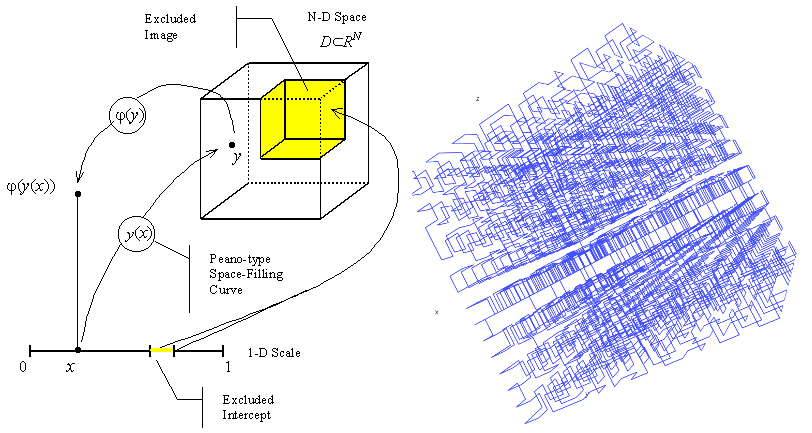
\includegraphics[scale=1.27]{images/peano.png}
              \end{figure}
              \end{minipage}

            \end{block}
        \end{column}
        \begin{column}[t]{0.48\paperwidth}
          \begin{block}{Параллельные версии метода оптимизации}
            Существует несколько способов распареллеливания алгоритма глобального поиска (АГП):
            \begin{itemize}
              \justifying
              \item Распараллеливание по характеристикам в рамках системы с общей памятью.
              На шаге 2 вместо одного интервала выбираются \(p\) интервалов с наилучшими характеристиками и в них параллельно проводятся испытания.
              \item Распараллеливание по развёрткам в рамках системы с раздельной памятью. На каждом узле системы работает копия метода, использующая
              уникальную развёртку. Копии метода обмениваются многомерными точками, однако одномерные прообразы этих точек различны для каждого метода.
              При использовании \(L\) развёрток каждый метод дополнительно получает \(L-1\) точку в свою поисковую информацию на каждой итерации, что
              ускоряет его сходимость.
              \item Сочетание указанных выше подходов.
            \end{itemize}
          В \cite{optParallelBook} перечисленные схемы описаны более подробно.
          \end{block}
          \begin{block}{Результаты}
            В таблице \ref{tab:parallelResults} приведены результаты применения распараллеливания по характеристикам, а также
            результаты, полученные при использовании комбинированного подхода с двумя развёртками.
            Поскольку размерность задачи оптимизации невелика, добавление дополнительных развёрток не привело к ускорению.

            \begin{table}[h]
            \caption{Результаты параллельных запусков на двух узлах кластера}
            \label{tab:parallelResults}
            \begin{tabular}{c|cccc}
              $L$ & $p=1$  & $p=2$ & $p=4$ & $p=8$\\
              \hline
              1  &  75,09 (1) & 59,58 (1,26) & 39.60 (1,89) & 12.28 (6,11) \\
              2  &  58,55 (1,28) & 46,14 (1,62) & 18.09 (4,15) & 9.21 (8,15) \\
              \hline
            \end{tabular}
            \end{table}

            Достигнутым практическим результатом является построение парето границы на плоскости критериев (рис. \ref{fig:pareto}).
            \begin{figure}
                \label{fig:pareto}
                \centering
                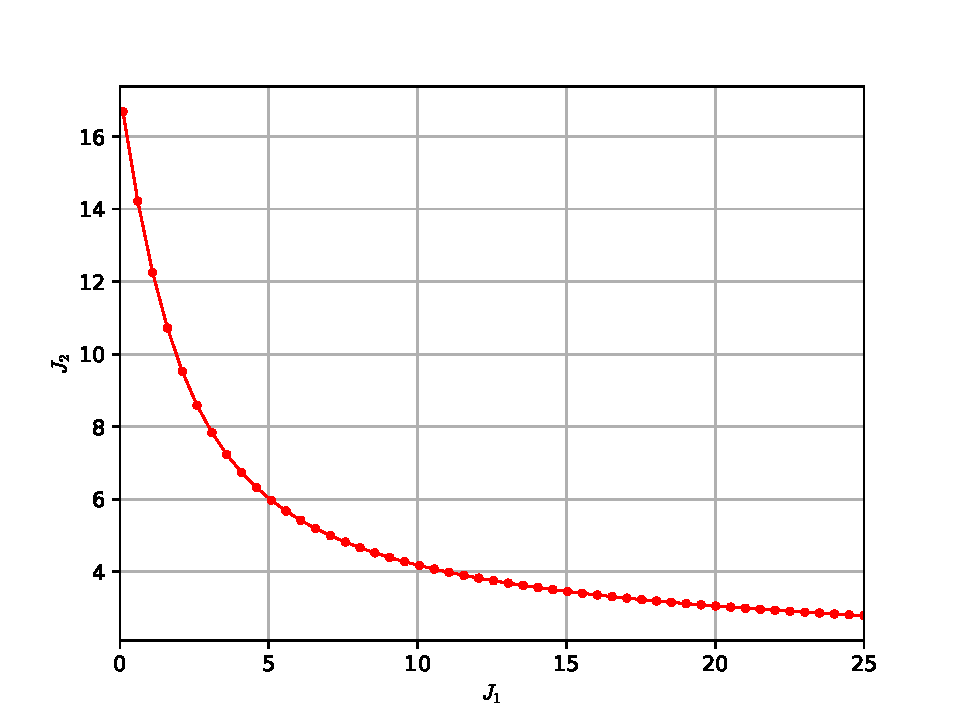
\includegraphics[scale=1.2]{images/solution.pdf}
                \caption{Парето-граница на плоскости критериев}
            \end{figure}
          \end{block}
          \begin{block}{Дальнейшая работа}
            В процессе решения задачи выяснилось, что критерии обладают большой константой Липшица вблизи границы устойчивости системы, что затрудняет оптимизацию и
            приводит к нестабильности результатов параллельных методов. Для решения этой проблемы требуется изменение решающих првил одномерного метода.
          \end{block}
          \begin{block}{Литература}
            \printbibliography
          \end{block}
        \end{column}
    \end{columns}
\end{frame}
\end{document}
